\documentclass[11pt, letterpaper, twoside]{book} % or scrreprt / report

% 1. Convert Beamer frame/slide commands into book paragraphs
\usepackage{beamerarticle}
\usepackage[margin=1in]{geometry}
\usepackage{hyperref}
\usepackage{amsmath, amssymb, amsthm}
\usepackage{booktabs}

% 3. Optional: Customize Chapter / Section headings
% \usepackage{titlesec}

% Import shared commands, packages, and custom macros
%
% Put stuff here that will be used for everything
\usepackage{tikz}
\usetikzlibrary{shapes,arrows.meta,positioning,plotmarks,shapes.misc} 
\usepackage{graphicx}
\graphicspath{
	{../lectures/images/}
	{../lectures/code/}
	}
\usepackage{natbib}
\usepackage{tcolorbox}
\usepackage{environ} % Required for handling environment bodies safely

% --- 1. DEFINE UNBREAKABLE BOX STYLING ---
\tcbset{
	slidebox/.style={
		colframe=black,        % Border color
		colback=white,         % Box background color
		arc=2mm,               % Rounded corners
		boxrule=0.5mm,         % Thickness of border
		width=\textwidth,      % Fit perfectly to text block width
		before=\vspace{1em},   % Spacing above the slide
		after=\vspace{1em}     % Spacing below the slide
	}
}

% --- 2. DEFINE THE WRAPPER ENVIRONMENT ---
% This safely captures everything inside the frame and renders it into a single, unbreakable box
\NewEnviron{sframe}[1]{%
	\begin{center}
		\begin{tcolorbox}[slidebox]
			{\large\bfseries #1}\par\medskip % Formatted Slide Title
			\BODY                            % Actual slide content
		\end{tcolorbox}
	\end{center}
}

% --- 3. REDIRECT BEAMER FRAMES TO THE SAFE ENVIROMENT ---
% In article mode, we redefine \begin{frame} to use our safe sframe tool
	\mode<article>{
		\let\frame\sframe
		\let\endframe\endsframe
	}


% Process only one chapter worth of notes
\includeonly{../lectures/lecture-02.tex}

\title{\textbf{Sustainability Economics: Complete Lecture Notes}}
\author{John Janmaat \\ \small Economics, Philosophy and Political Science, The University of British Columbia}
\date{Academic Year 2026--2027}

\begin{document}
	
	\frontmatter
	\maketitle
	\tableofcontents
	
	\chapter*{Course Overview \& Syllabus Summary}
	\addcontentsline{toc}{chapter}{Course Overview \& Syllabus Summary}
	What is the connection between economics and sustainability?  When people talk about economics, often they are talking about something to do with money.  How people acquire it and what they do with it.  When people talk about sustainability, often they are talking about the environment, how it is changing, and whether or not those changes are good.  Where do these two things come together?  That intersection often seems to be about the way that people are acquiring and using money is changing the environment in ways that are not good.
	
	\mainmatter
	
	% ==========================================
	% PART I: FOUNDATIONS
	% ==========================================
	\part{Foundations \& Basic Principles}
	
	\chapter{Introduction \& Key Concepts}
	%! TEX root = ../notes/main_notes.tex

\lecture{Introduction to the Course}{lec-01}

% Only appears in book/notes mode
\mode<article>{
	\section{Overview \& Objectives}
	The term \emph{sustainability} implies continuity and balance.  If something is sustainable, it can continue doing what it is doing.  Unless it is doing nothing, what it is doing is interacting with other entities.  This implies that, except for those things that are doing nothing, we should think about sustainability with a systems perspective.
	
	A system is a collection of entities (or elements) and the connections between them.  To understand a system, we need to understand the entities and their connections.  Our goal in this course is to develop an understanding of the relationship between the economy and the environment by looking at the elements that make up the economy and their relationship with elements that make up the environment.  To do so, we will proceed by building a model of a \emph{complex adaptive social ecological system}. 
	
	The system we inhabit, and that we will try to understand, is complex.  This means that the system as a whole exhibits properties that cannot be explained by looking at any element itself.  It is adaptive in that it changes in response to internal and external pressures.
	
	\begin{note}
		Key reading for this section: Chapter 1 of the required textbook.
	\end{note}
}

% Frame 1

\begin{frame}{Systems}
	% \begin{columns}
		% \column{0.6\textwidth}
			\begin{itemize}
				\item A system is a collection of elements and their connections.
				\item A social ecological system contains elements in both the social (human) and ecological (nature) domains, and has connections crossing between the domains.
				\item A system is complex when there are 'emergent' properties that cannot be predicted looking at elements in isolation.
				\item A system is adaptive if it continuously evolves or changes in response to internal and external forces.
			\end{itemize}
		% \column{0.4\textwidth}
		% 	\centering
		%	
\includegraphics{SESgraphic.png}
	% \end{columns}
\end{frame}

\begin{frame}{Systems}
	\centering
	\includegraphics<presentation>[width=0.6\linewidth]{SESgraphic.png}
	\includegraphics<article>[width=0.8\linewidth]{SESgraphic.png}
\end{frame}


% Interspersed notes text between slides
\mode<article>{
	\subsection{Systems and Subsystems}
	The global social ecological system is far too complex for anyone to comprehend.  At present, it is probably too complex for AI to comprehend as well.  What both humans and AI do with this is focus on a part of the system that we are interested in.  We choose a boundary and a scale.  Things beyond the boundary are grouped together into subsystems, the internal details of which are not considered.  This would be at the scale that is coarser than the part of the system we are interested in.  For those things at a finer scale, we also relegate those things into subsystems, with the entire subsystem being taken as an element of the system we are studying.
	
	The concerns about sustainability can be seen as concerns about the details that are being left out.
	
	
}

\begin{frame}{Production Possibilities}
	\begin{columns}[T]
		\begin{column}{0.3\textwidth}
			\begin{itemize}
				\item What is missing?
			\end{itemize}
		\end{column}
		\begin{column}{0.7\textwidth}
			\centering
			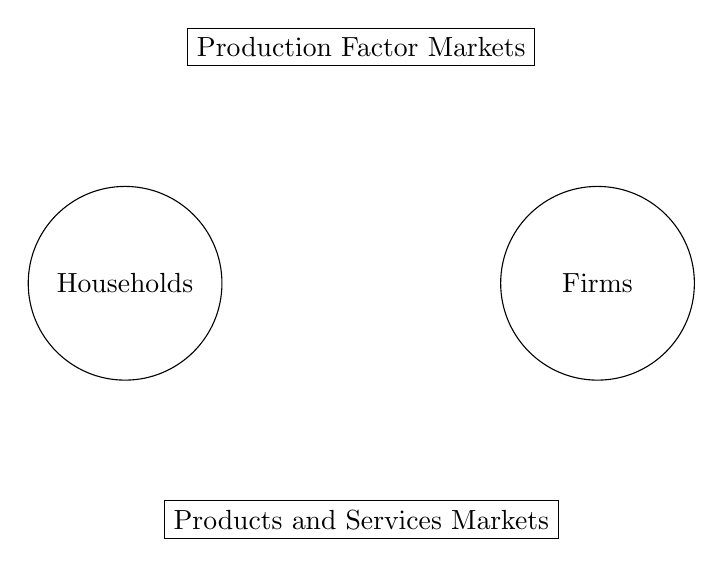
\begin{tikzpicture}
				\node [rectangle, draw] at (3,6) {Production Factor Markets};
				\node [rectangle, draw] at (3,0) {Products and Services Markets};
				\node [circle, draw, minimum size=70pt] at (0,3) {Households};
				\node [circle, draw, minimum size=70pt] at (6,3) {Firms};
			\end{tikzpicture}
		\end{column}
	\end{columns}
\end{frame}

	
	\chapter{Systems}
	%! TEX root = ../notes/main_notes.tex

\lecture{The Physical System}{lec-01}

% Only appears in book/notes mode
\mode<article>{
	\section{Systems}
	A system is a collection of entities (or elements) and the connections between them.  To understand a system, we need to understand the entities and their connections.  Our goal in this course is to develop an understanding of the relationship between the economy and the environment by looking at the elements that make up the economy and their relationship with elements that make up the environment.  To do so, we will proceed by building a model of a \emph{complex adaptive social ecological system}. 
	
	The system we inhabit, and that we will try to understand, is complex.  This means that the system as a whole exhibits properties that cannot be explained by looking at any element itself.  It is adaptive in that it changes in response to internal and external pressures.
	
	\begin{note}
		Something of note.
	\end{note}
}

% Frame 1
\begin{frame}{Systems}
	% \begin{columns}
		% \column{0.6\textwidth}
			\begin{itemize}
				\item A system is a collection of elements and their connections.
				\item A social ecological system contains elements in both the social (human) and ecological (nature) domains, and has connections crossing between the domains.
				\item A system is complex when there are 'emergent' properties that cannot be predicted looking at elements in isolation.
				\item A system is adaptive if it continuously evolves or changes in response to internal and external forces.
			\end{itemize}
		% \column{0.4\textwidth}
		% 	\centering
		%	
\includegraphics{SESgraphic.png}
	% \end{columns}
\end{frame}

\begin{frame}{Systems}
	\centering
	\includegraphics<presentation>[width=0.6\linewidth]{SESgraphic.png}
	\includegraphics<article>[width=0.8\linewidth]{SESgraphic.png}
\end{frame}

% Interspersed notes text between slides
\mode<article>{
	When we think about systems, we need to consider scale.  If we consider the scale of ...
}

% Frame 2
\begin{frame}{Scales}
	\begin{itemize}
		\item What constitutes elements of a system depends on the physical scale at which we are contemplating the system.
		\begin{itemize}
			\item At the atomic scale, atoms are the elements.
			\item At the cosmic scale, galaxies are the elements.
			\item What are the elements at the human scale?
		\end{itemize}	
		\item What the connections between elements are depends on the physical scale and the temporal scale chosen.
		\begin{itemize}
			\item How long does it take for the connection to change something for the elements that we are interested in?
			\item For the movement of atoms ...
			\item For the movement of galaxies ...
			\item For the human issues we are concerned about?
		\end{itemize}
	\end{itemize}
\end{frame}

\mode<article>{
	In both the natural and social systems, researchers try to identify patterns in the systems that they are studying.  Those patterns emerge from the interactions between the elements that make up the system.  When systems are large and complex, the discipline typically finds ways to describe the patterns without examining the detail of the interacting entities that leads to the pattern.
	
	Cosmologists studying the movement of galaxies do not spend much time considering the movement of individual hydrogen atoms.  However, it is the movement of those individual hydrogen atoms, under the influence of gravity, that leads to the formation of stars, and that leads to stars spinning together in galaxies.
	
	Often, the disciplines have observed or thought deeply about the entities that they are interested in, and arrived at relationships - often mathematical - that represent the patterns that they observe.
	
	In chemistry, the relationship $PV = nRT$ is known at the Ideal Gas Law.  It is the relationship between pressure ($P$), volume ($V$) and temperature ($T$).  The amount of gas in the volume is ($n$) in units of moles, and $R$ is the ideal gas constant, expressed the the appropriate units.  A mole is Avagadro's number of atoms.  This relationship expresses how temperature, which is a measure of how much energy atoms have, and the pressure that they are exerting within a particular volume.  The physics of the situation is that the atoms are racing around, their speed reflecting the temperature, and smashing into the sides of the container that confines them.  The more energy they have, the faster they are moving, and the harder they collide with the chamber.  However, the equation is not representing the movement of those individual atoms.  Rather, it is expressing this effect in a way that is relevant for things like the operation of a steam engine.
	
	In the last few decades, computers have become powerful enough for us to represent the details of relationships like this from the basic building blocks.  Agent based models are a class of such tools.  One such agent based modeling environment we will use from time to time is NetLogo (https://www.netlogo.org/).  
}

\begin{frame}{Agent Based Models}
	\begin{itemize}
		\item Agent Based Models (ABMs) that interact virtual agents in virtual environments, ot observe how the system evolves.
		\item Agents can range from individual atoms to galaxies.
	\end{itemize}
\end{frame}

\mode<article>{
	When people who are concerned about the environment think of economics, they often conclude that it ignores the environment.  The way introductory economics is taught often reinforces this, as if the environment is mentioned at all, it is a small topic, externalities.
	
	There is a practical reason for this.  During a presidential debate, former US president Bill Clinton said "It's the economy, stupid." [CONFIRM QUOTE].  He was emphasizing that what people are most worried about is their own situation.  In a modern economy, your situation depends on your income and what it costs you to live.  The environment is important, but is secondary to being able to put food on the table tonight, and having a roof under which that table is placed.
	
	You are in this course because you are concerned about the environment, about sustainability.  Therefore, lets start by building our understanding of sustainability economics from that environment.
}

\begin{frame}{The Fish Pond}
	\begin{itemize}
		\item The Question: How does the population of fish in a pond change over time?
		\begin{itemize}
			\item What time step?
			\item One minute? - population changes small, unless major event.
			\item One century? - population change in relation to long term events.
			\item One year? - scale that matches seasons.
		\end{itemize}
		\item The elements of a fish pond.
		\begin{itemize}
			\item The fish (each fish, or fish as a population - biomass?).
			\item The water (each molecule, or as a medium for the fish?).
			\item The food (each food item - e.g phytoplankton, insects, other fish - or as a population - biomass?).
		\end{itemize}	
		\item The connections within the fish pond system.
		\begin{itemize}
			\item Fish encountering food and eating.
			\item Fish health and survival affected by state of the water.
			\item Fish encounter each other and reproduce.
		\end{itemize}
	\end{itemize}
\end{frame}

\mode<article>{
	In both the natural and social systems, researchers try to identify patterns in the systems that they are studying.  Those patterns emerge from the interactions between the elements that make up the system.  When systems are large and complex, the discipline typically finds ways to describe the patterns without examining the detail of the interacting entities that leads to the pattern.
	
	Cosmologists studying the movement of galaxies do not spend much time considering the movement of individual hydrogen atoms.  However, it is the movement of those individual hydrogen atoms, under the influence of gravity, that leads to the formation of stars, and that leads to stars spinning together in galaxies.
	
	Often, the disciplines have observed or thought deeply about the entities that they are interested in, and arrived at relationships - often mathematical - that represent the patterns that they observe.
	
	In chemistry, the relationship $PV = nRT$ is known at the Ideal Gas Law.  It is the relationship between pressure ($P$), volume ($V$) and temperature ($T$).  The amount of gas in the volume is ($n$) in units of moles, and $R$ is the ideal gas constant, expressed the the appropriate units.  A mole is Avagadro's number of atoms.  This relationship expresses how temperature, which is a measure of how much energy atoms have, and the pressure that they are exerting within a particular volume.  The physics of the situation is that the atoms are racing around, their speed reflecting the temperature, and smashing into the sides of the container that confines them.  The more energy they have, the faster they are moving, and the harder they collide with the chamber.  However, the equation is not representing the movement of those individual atoms.  Rather, it is expressing this effect in a way that is relevant for things like the operation of a steam engine.
	
	In the last few decades, computers have become powerful enough for us to represent the details of relationships like this from the basic building blocks.  Agent based models are a class of such tools.  One such agent based modeling environment we will use from time to time is NetLogo (https://www.netlogo.org/).  
}
\mode<article>{
	
	Fish example: https://virtualbiologylab.org/ModelsHTML5/PopGenFishbowl/PopGenFishbowl.html 
}
	
	
	% ==========================================
	% PART II: ADVANCED TOPICS
	% ==========================================
	\part{Foundational Systems}
	
	\chapter{Social Ecological Systems \#1}
	%! TEX root = ../notes/main_notes.tex

\lecture{A Foundational Ecological System}{lec-systems}

\mode<article>{
	When people who are concerned about the environment think of economics, they often conclude that it ignores the environment.  The way introductory economics is taught often reinforces this, as if the environment is mentioned at all, it is a small topic, externalities.
	
	There is a practical reason for this.  During a presidential debate, former US president Bill Clinton said "It's the economy, stupid." [CONFIRM QUOTE].  He was emphasizing that what people are most worried about is their own situation.  In a modern economy, your situation depends on your income and what it costs you to live.  The environment is important, but is secondary to being able to put food on the table tonight, and having a roof under which that table is placed.
	
	You are in this course because you are concerned about the environment, about sustainability.  Therefore, lets start by building our understanding of sustainability economics from that environment.
}

\begin{frame}{The Fish Pond}
	\begin{itemize}
		\item The Question: How does the population of fish in a pond change over time?
		\begin{itemize}
			\item What time step?
			\item One minute? - population changes small, unless major event.
			\item One century? - population change in relation to long term events.
			\item One year? - scale that matches seasons.
		\end{itemize}
		\item The elements of a fish pond.
		\begin{itemize}
			\item The fish (each fish, or fish as a population - biomass?).
			\item The water (each molecule, or as a medium for the fish?).
			\item The food (each food item - e.g phytoplankton, insects, other fish - or as a population - biomass?).
		\end{itemize}	
		\item The connections within the fish pond system.
		\begin{itemize}
			\item Fish encountering food and eating.
			\item Fish health and survival affected by state of the water.
			\item Fish encounter each other and reproduce.
		\end{itemize}
	\end{itemize}
\end{frame}

\mode<article>{
	In both the natural and social systems, researchers try to identify patterns in the systems that they are studying.  Those patterns emerge from the interactions between the elements that make up the system.  When systems are large and complex, the discipline typically finds ways to describe the patterns without examining the detail of the interacting entities that leads to the pattern.
	
	Cosmologists studying the movement of galaxies do not spend much time considering the movement of individual hydrogen atoms.  However, it is the movement of those individual hydrogen atoms, under the influence of gravity, that leads to the formation of stars, and that leads to stars spinning together in galaxies.
	
	Often, the disciplines have observed or thought deeply about the entities that they are interested in, and arrived at relationships - often mathematical - that represent the patterns that they observe.
	
	In chemistry, the relationship $PV = nRT$ is known at the Ideal Gas Law.  It is the relationship between pressure ($P$), volume ($V$) and temperature ($T$).  The amount of gas in the volume is ($n$) in units of moles, and $R$ is the ideal gas constant, expressed the the appropriate units.  A mole is Avagadro's number of atoms.  This relationship expresses how temperature, which is a measure of how much energy atoms have, and the pressure that they are exerting within a particular volume.  The physics of the situation is that the atoms are racing around, their speed reflecting the temperature, and smashing into the sides of the container that confines them.  The more energy they have, the faster they are moving, and the harder they collide with the chamber.  However, the equation is not representing the movement of those individual atoms.  Rather, it is expressing this effect in a way that is relevant for things like the operation of a steam engine.
	
	In the last few decades, computers have become powerful enough for us to represent the details of relationships like this from the basic building blocks.  Agent based models are a class of such tools.  One such agent based modeling environment we will use from time to time is NetLogo (https://www.netlogo.org/).  
}
\mode<article>{
	
	Fish example: https://virtualbiologylab.org/ModelsHTML5/PopGenFishbowl/PopGenFishbowl.html 
}

\begin{frame}{The Fish Pond}
	\centering
	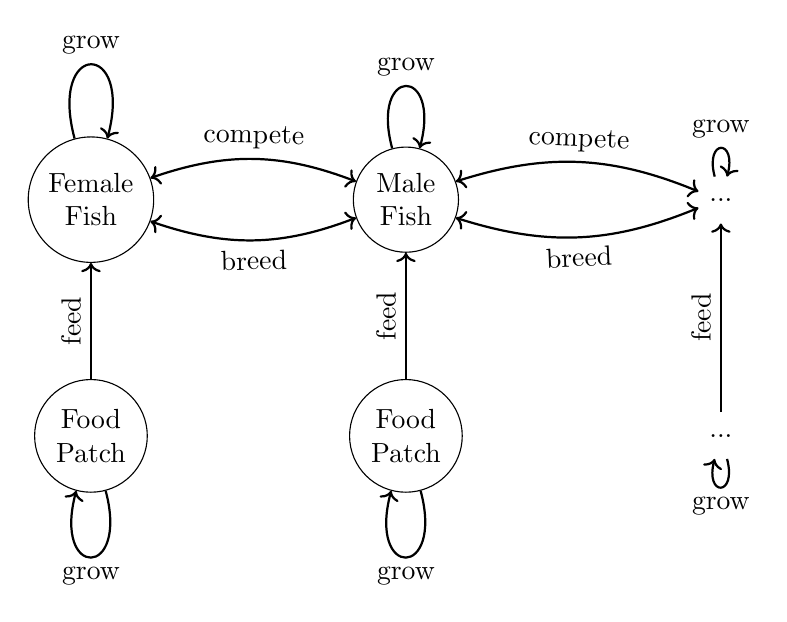
\begin{tikzpicture}
		% Define and place the nodes
		\node [circle, draw, align=center] at (2,5) (fish1) {Female \\ Fish};
		\node [circle, draw, align=center] at (6,5) (fish2) {Male \\ Fish};
		\node [circle] at (10,5) (fish3) {...};
		\node [circle, draw, align=center] at (2,2) (patch1) {Food \\ Patch};
		\node [circle, draw, align=center] at (6,2) (patch2) {Food \\ Patch};
		\node [circle] at (10,2) (patch3) {...};
		
		% Draw edges
		\draw [->, thick] (patch1) to [bend left=0] node [above, sloped] {feed} (fish1);
		\draw [->, thick] (patch2) to [bend left=0] node [above, sloped] {feed} (fish2);
		\draw [->, thick] (patch3) to [bend left=0] node [above, sloped] {feed} (fish3);
		\draw [<->, thick] (fish1) to [bend left=20] node [above, sloped] {compete} (fish2);
		\draw [<->, thick] (fish1) to [bend left=-20] node [below, sloped] {breed} (fish2);
		\draw [<->, thick] (fish2) to [bend left=20] node [above, sloped] {compete} (fish3);
		\draw [<->, thick] (fish2) to [bend left=-20] node [below, sloped] {breed} (fish3);
		\draw [->, thick] (fish1) to [loop above] node[above, sloped] {grow} (fish1);
		\draw [->, thick] (fish2) to [loop above] node[above, sloped] {grow} (fish2);
		\draw [->, thick] (fish3) to [loop above] node[above, sloped] {grow} (fish3);
		\draw [->, thick] (patch1) to [loop below] node[below, sloped] {grow} (patch1);
		\draw [->, thick] (patch2) to [loop below] node[below, sloped] {grow} (patch2);
		\draw [->, thick] (patch3) to [loop below] node[below, sloped] {grow} (patch3);
		% \draw [->, thick] (lake) to[bend left=20] node[above, sloped] {fish} (hermit);
		% \draw [->, thick] (field) to[bend right=20] node[above, sloped] {sediment} (lake);
	\end{tikzpicture}
\end{frame}

\begin{frame}{The Fish Pond}
	\begin{itemize}
		\item What question(s) are we trying to answer with a model?
		\item What features of the elements (fish and food patches) and their interactions will lead to a sustainable system.
		\begin{itemize}
			\item Sustainable = does not collapse to a system without fish.
		\end{itemize}
		\item What level of harvest is sustainable?
		\begin{itemize}
			\item Sustainable = harvest level that can continue without collapsing system to one without fish.
		\end{itemize}
		\item How much detail do we need to model about the ecological system to identify the sustainable harvest level?
		\begin{itemize}
			\item Can elements of fish pond system be treated together as one element of a social-ecological system?
			\item Is the internal workings of the fish pond subsystem necessary to identify sustainable harvest levels?
		\end{itemize}
	\end{itemize}
\end{frame}

\begin{frame}{The Fish Pond}
	\begin{itemize}
		\item A NetLogo model.
		\item Fish (agents) swim around in pond with patches (environment) where they feed.
		\begin{itemize}
			\item Fish: age to breeding, lifespan, how much food, impact of competition, breeding behavior, movement, ...
			\item Food patch: how much food, growth rate of food.
		\end{itemize}
		\item Lots of details that can be considered.
		\item Do we loose sight of the forest by focusing too much on the trees?
	\end{itemize}
\end{frame}

\begin{frame}{The Fish Pond}
	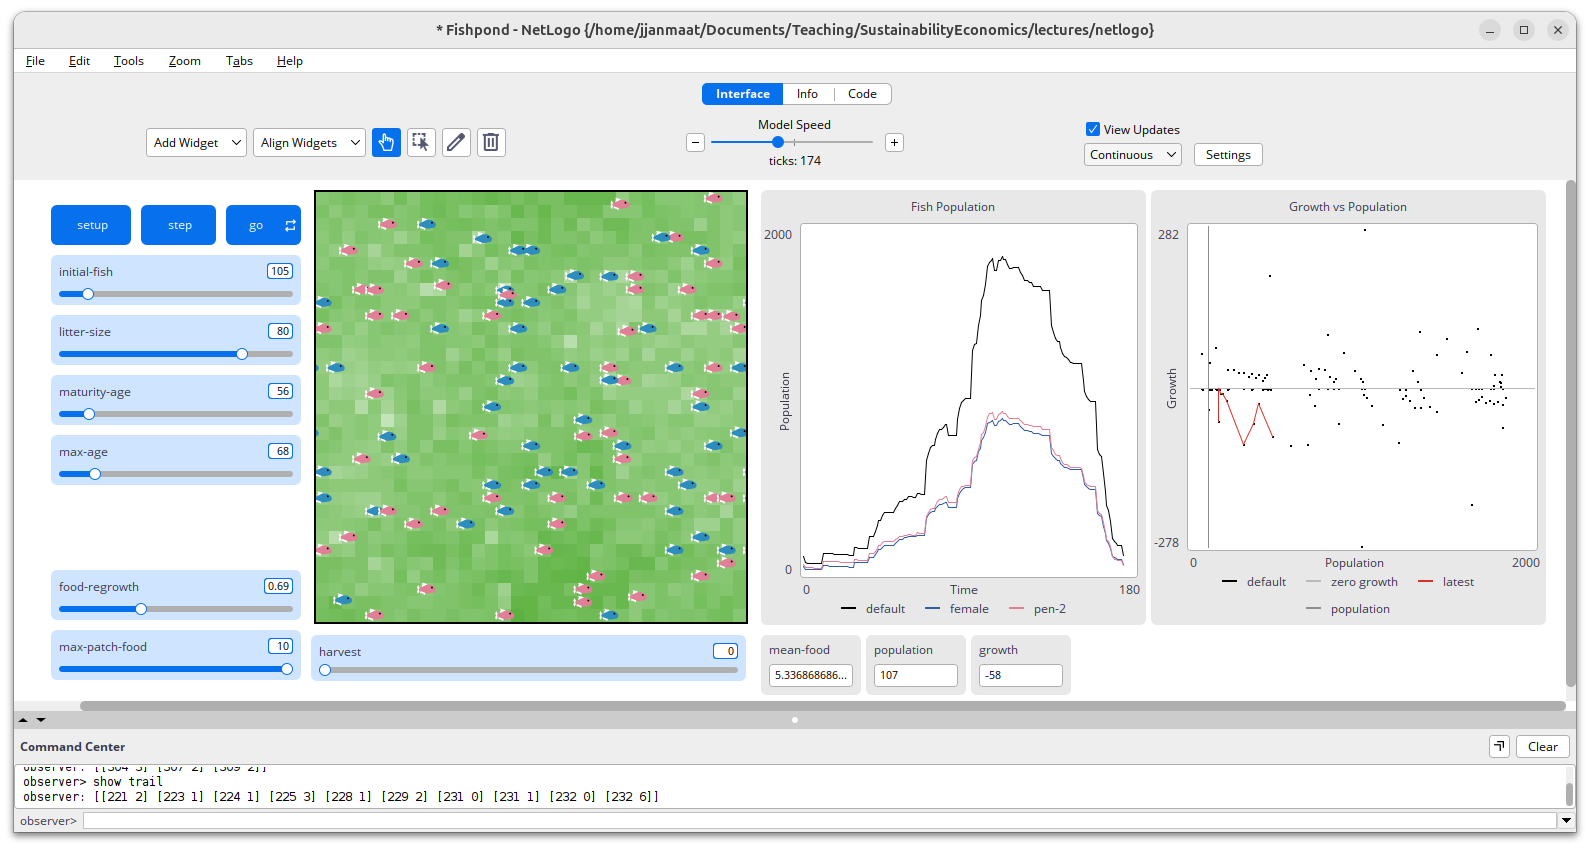
\includegraphics[width=1.0\textwidth]{NetLogoFishPond1.png}
\end{frame}

\begin{frame}{Fishing in the Pond}
	\begin{itemize}
		\item Fish harvester chooses how much effort (e.g. time) to spend fishing.
		\item Most processes in pond not affected by amount of fishing effort.
		\item Effects of harvesting:
		\begin{itemize}
			\item Reduces population of fish.
			\item Reduces fish on fish competition - increasing growth.
			\item Increases success of reproduction.
			\item May force population so low that collapses.
		\end{itemize}
		\item Harvest effort:
		\begin{itemize}
			\item With same effort, more fish caught if more fish in pond.
		\end{itemize}
	\end{itemize}
\end{frame}

\begin{frame}{Fishing in the Pond}
	\centering
	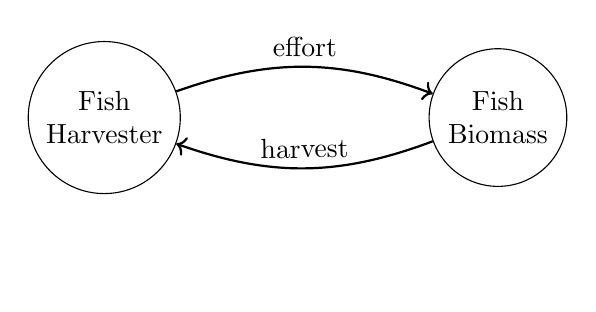
\begin{tikzpicture}
		\node [circle, draw, align=center] at (1,3) (harvester) {Fish \\ Harvester};
		\node [circle, draw, align=center] at (6,3) (population) {Fish \\ Biomass};
		\node at (1,1) {};
		
		\draw [->, thick] (harvester) to [bend left=20] node [above, sloped] {effort} (population);
		\draw [->, thick] (population) to [bend left=20] node [above, sloped] {harvest} (harvester);
	\end{tikzpicture}
	\begin{itemize}
		\item What effort level will result in a sustainable harvest?
	\end{itemize}
\end{frame}

\begin{frame}{Fishing in the Pond}
	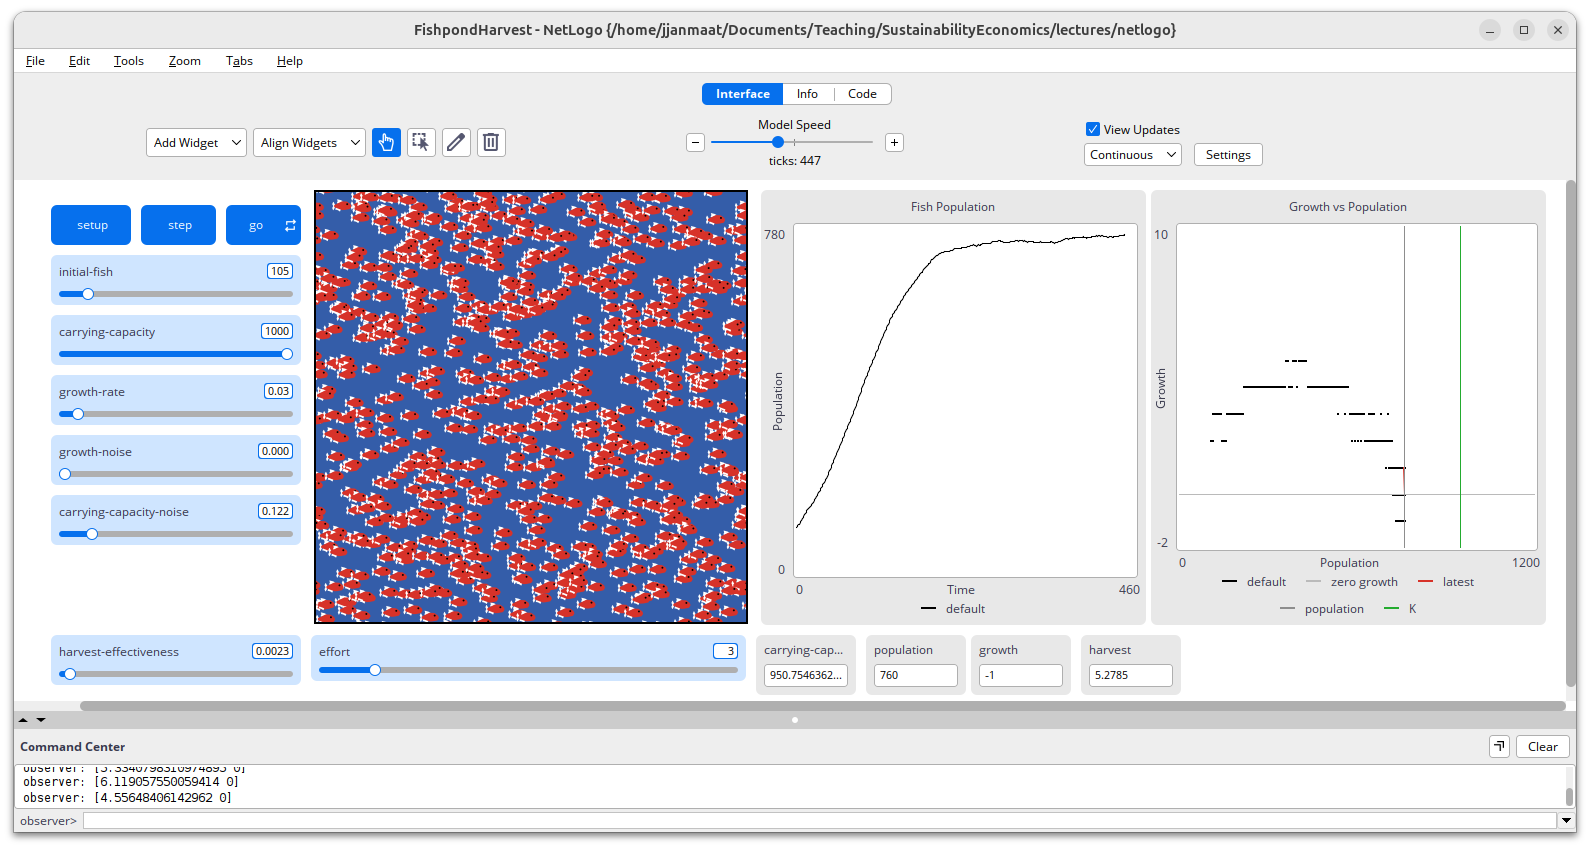
\includegraphics[width=1.0\textwidth]{NetLogoFishPond2.png}
\end{frame}

\begin{frame}{Fishy Math}
	\begin{itemize}
		\item Fish population modeled with logistic growth curve.
		\[
		\frac{\Delta N}{\Delta t} = rN\left(1 - \frac{N}{K}\right) = \frac{\partial N}{\partial t} = \dot{N}
		\]
		\begin{itemize}
			\item $\Delta N$ is change in fish population during time interval $\Delta t$.
			\item $N$ is fish population.
			\item $r$ is rate of growth of fish population.
			\item $K$ is carrying capacity of the ecosystem represented by the model.
		\end{itemize}
	\end{itemize}
\end{frame}

\begin{frame}{Fishy Math}
	\begin{tikzpicture}
		\draw [-] (0,0) to node [below, yshift=-8pt] {Population ($N$)} (11,0);
		\draw [-] (0,0) to node [above, sloped, yshift=8pt] {Growth ($\Delta N / \Delta t$)} (0,6);
		\draw [domain=0:10, smooth, variable=\N] plot ({\N},{4*(0.5*\N*(1-\N/10))});
		\node [below, align=center] at (10,0) {$10$ \\ $K$};
		\node [below] at (0,0) {0};
		\node [left] at (0,0) {0};
		\node [left] at (0,4) {1};
		\node [right, align=left] at (7,5.5) {$\dfrac{\Delta N}{\Delta t} = 0.5N \left(1 - \dfrac{N}{10}\right)$};
	\end{tikzpicture}
\end{frame}

\begin{frame}{Fish Production Function}
	\begin{itemize}
		\item In economics, a \textbf{\textit{technology}} refers to a process that transforms \textit{\textbf{inputs}} into \textit{\textbf{outputs}}.
		\item A function that describes this process is called a \textit{\textbf{production function}}.
		\item In this example, effort is the input, and harvest is the output.
		\[
		H = qEN
		\]
		\begin{itemize}
			\item $H$ is the harvest.
			\item $E$ is the effort.
			\item $N$ is the population of fish.
			\item $q$ measures how catchable the fish are.
		\end{itemize}
		\item Note that the productivity of fishing effort depends on the size of fish population (the stock).
		\item A unit of effort $E$ harvests a fraction $q$ of the stock $N$.
	\end{itemize}
\end{frame}

\begin{frame}{Fish Production Function}
	\begin{itemize}
		\item There are three measures that are commonly used in economics to describe aspects of the production process.
		\begin{enumerate}
			\item \textit{\textbf{Total Product (TP)}} is the total output at a particular input level $X$. 
			\item \textit{\textbf{Average Product (AP)}} is the total output at a particular level of input, divided by that level of input.
			\[
			AP = \frac{TP}{X}
			\]
			\item \textit{\textbf{Marginal Product (MP)}} is, at a particular level of an input, the amount by which output will increase for a small increase in that input.
			\[
			MP = \frac{\Delta TP}{\Delta X} = \frac{\partial TP}{\partial X}
			\]
			\begin{itemize}
				\item The marginal product is the slope of the total product at $X$.
			\end{itemize}
		\end{enumerate}
	\end{itemize}
\end{frame}

\begin{frame}{Fish Production Function}
	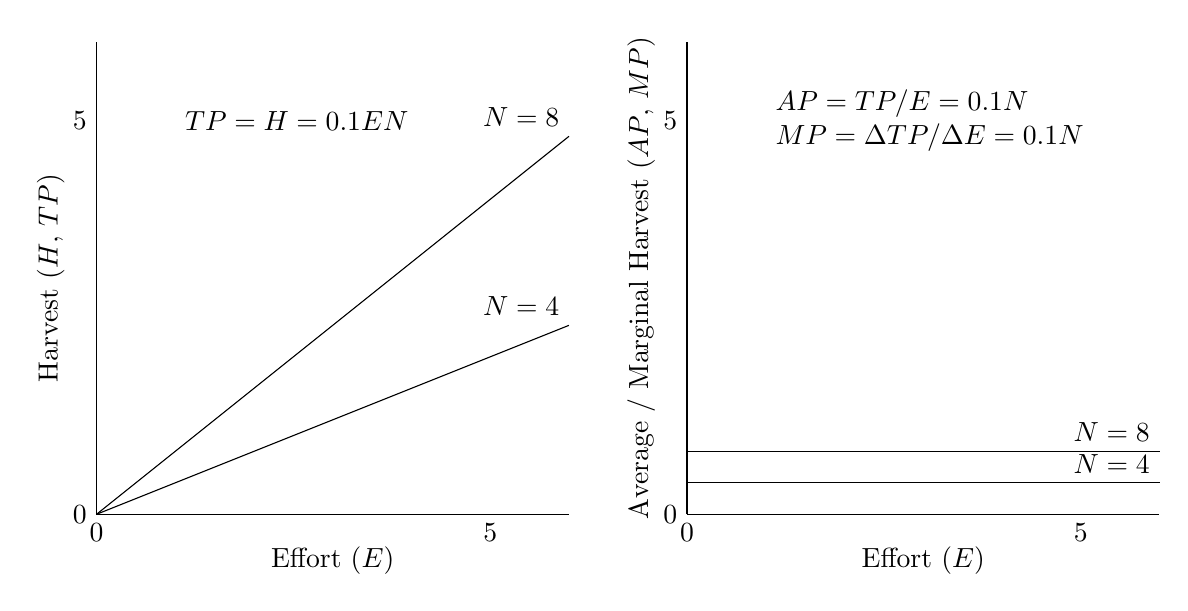
\begin{tikzpicture}
		\draw [-] (0,0) to node [below, yshift=-8pt] {Effort ($E$)} (6,0);
		\draw [-] (0,0) to node [above, sloped, yshift=8pt] {Harvest ($H$, $TP$)} (0,6);
		\draw [-] (7.5,0) to node [below, yshift=-8pt] {Effort ($E$)} (13.5,0);
		\draw [-] (7.5,0) to node [above, sloped, yshift=8pt] {Average / Marginal Harvest ($AP$, $MP$)} (7.5,6);
		\draw plot [domain=0:6, smooth, variable=\E] ({\E},{0.1*\E*8}) node [above left] {$N = 8$};
		\draw plot [domain=0:6, smooth, variable=\E] ({\E},{0.1*\E*4}) node [above left] {$N = 4$};
		\draw plot [domain=7.5:13.5, smooth, variable=\E] ({\E},{0.1*8}) node [above left] {$N = 8$};
		\draw plot [domain=7.5:13.5, smooth, variable=\E] ({\E},{0.1*4}) node [above left] {$N = 4$};
		\node [right] at (1,5) {$TP = H = 0.1EN$};
		\node [right, align=left] at (8.5,5) {$AP = TP / E = 0.1N$ \\ $MP = \Delta TP / \Delta E = 0.1N$};
		\node [left] at (0,0) {0};
		\node [below] at (0,0) {0};
		\node [left] at (7.5,0) {0};
		\node [below] at (7.5,0) {0};
		\node [left] at (0,5) {5};
		\node [below] at (5,0) {5};
		\node [left] at (7.5,5) {5};
		\node [below] at (12.5,0) {5};
	\end{tikzpicture}
\end{frame}

\mode<article>{
	The average and marginal product are the same for this production function.  Given a particular fish population, each unit of effort catches the same number of fish.  This would stop when there are no more fish left. For the range over which effort is shown in the figure, this does not happen.
	
	Suppose the harvester is deciding how much effort to exert this period, which we will call a year.  It is important to recognize that the choice of effort this year affects how many fish will be available to be caught next year.  The fish that are left behind reproduce, and this reproduction adds to the supply of fish that can be caught next year.
	
	We can throw some numbers at the example to make it a bit more concrete.
}

\begin{frame}{Fish Production Function}
	\begin{itemize}
		\item Increasing effort increases harvest.
		\item Larger harvest means less fish left behind to reproduce.
		\item There is an \textit{\textbf{opportunity cost}} to catching more fish today in terms of the lost contribution to growth of the fish stock in the future.
	\end{itemize}
\end{frame}

\mode<article>{
	In the table below, the size of the fish stock, the amount harvested and the growth of the fish stock following harvest is shown for the first ten years, for effort levels $E = 2$ and $E = 3$.
	
	The sequence within a year is that first fish reproduce and then the harvest is taken.  What is left of the fish stock is the growth less the amount harvested.
	
	The numbers in the table show a clear trend.  For these two effort levels, the stock of fish and the harvest decrease over time.  For the lower effort, the beginning harvest is lower.  However, if this lower effort is maintained, then the lower harvest leads to a slower decline in the fish stock, and by the end of the ten years, the lower effort is resulting in a higher harvest than for the higher effort level.
	
	If you look closely at the numbers, you can see that the differences from one year to the next are getting smaller.  In each case, with the constant effort level, the system is converging on a \textit{\textbf{steady state}}.  At the steady state, the size of the stock, the amount that is harvested, and the amount by which the fish stock grows are constant.  In fact, the growth exactly matches the amount harvested.  Each of these steady states is in effect sustainable.  Which one do we like better?
}
\begin{frame}{Fish Production Function}
	$$H = 0.1EN\ \ \ \ \ \ \dfrac{\Delta N}{\Delta t} = 0.5N \left(1 - \dfrac{N}{10}\right) - H$$
	\vskip 12pt
	\centering
	\begin{tabular}{ccccccccccc}
		\hline
		$t$ &  $N$  & $E$ & $H$  & $\Delta N$ &  &  $N$  & $E$ & $H$  & $\Delta N$ &  \\ \hline
		 1  & 10.00 &  2  & 2.00 &    0.00    &  & 10.00 &  4  & 4.00 &    0.00    &  \\
		 2  & 8.00  &  2  & 1.60 &    0.80    &  & 6.00  &  4  & 2.40 &    1.20    &  \\
		 3  & 7.20  &  2  & 1.44 &    1.01    &  & 4.80  &  4  & 1.92 &    1.25    &  \\
		 4  & 6.77  &  2  & 1.35 &    1.09    &  & 4.13  &  4  & 1.65 &    1.21    &  \\
		 5  & 6.51  &  2  & 1.30 &    1.14    &  & 3.69  &  4  & 1.48 &    1.16    &  \\
		 6  & 6.34  &  2  & 1.27 &    1.16    &  & 3.38  &  4  & 1.35 &    1.12    &  \\
		 7  & 6.23  &  2  & 1.25 &    1.17    &  & 3.14  &  4  & 1.26 &    1.08    &  \\
		 8  & 6.16  &  2  & 1.23 &    1.18    &  & 2.96  &  4  & 1.19 &    1.04    &  \\
		 9  & 6.11  &  2  & 1.22 &    1.19    &  & 2.82  &  4  & 1.13 &    1.01    &  \\
		10  & 6.08  &  2  & 1.22 &    1.29    &  & 2.71  &  4  & 1.08 &    0.99    &  \\ \hline
	\end{tabular}
\end{frame}
\mode<article>{
	The following graphs show the progression of the stock as the continuing harvests change the size of the stock and the growth.
	
	The system starts at the carrying capacity $K$.  At the carrying capacity, the stock is steady.  The new fish added to the population, the recruitment, is exactly matched by the deaths.  There is no net growth of the stock.
	
	The first harvest reduces the stock by the amount of the harvest.  When the effort is lower, this harvest is lower.  As the stock is now below the carrying capacity, it has room to grow.  That growth is represented by the height of the curve.  
	
	The second harvest captures a quantity of fish equal to all the growth and a bit more, reducing the stock further.  This effect is larger for the case with the larger effort.  With the stock reduced further, there is more capacity for growth.
	
	In the figures, things begin to diverge with the third harvest.  When the effort is low, the change in the stock after the harvest leads to an increase in the growth of the stock.  However, when the effort is high, the stock has been depleted so much that the further depletion results in a lower growth rate.  We have moved the stock to a place where there is little competition for food, but it takes a lot of effort to find others to mate with.
	
	If we continue with the same effort levels, the systems will converge on a steady state.  The steady state is the level of the stock such that, given the effort level, that stock does not change any further.  In these examples, the higher effort level leads to a lower steady state stock and a lower steady state harvest than for the lower effort level.	
}

\begin{frame}{Fish Production Function}
	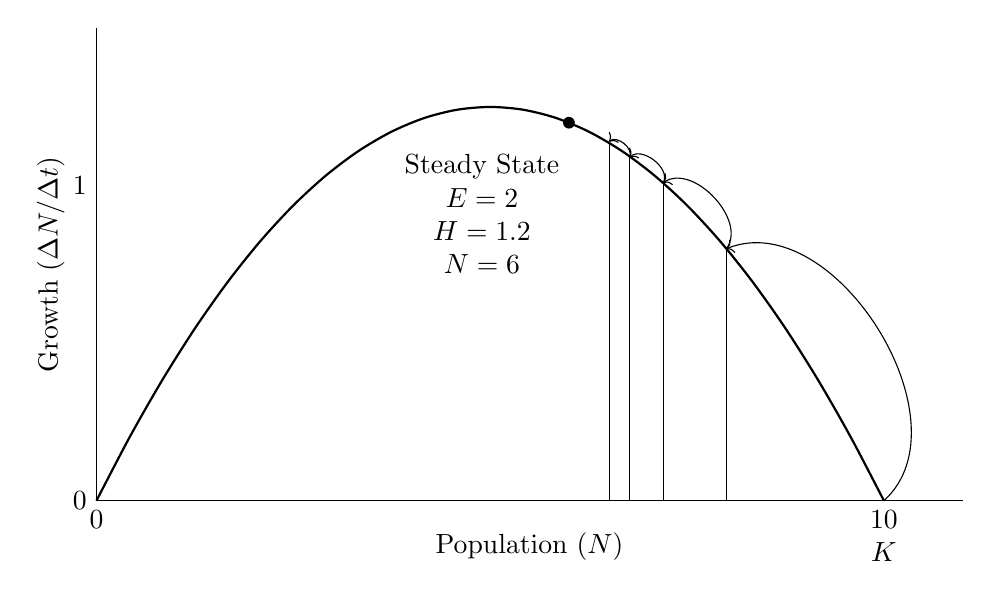
\begin{tikzpicture}
		\draw [-] (0,0) to node [below, yshift=-8pt] {Population ($N$)} (11,0);
		\draw [-] (0,0) to node [above, sloped, yshift=8pt] {Growth ($\Delta N / \Delta t$)} (0,6);
		\draw [thick, domain=0:10, smooth, variable=\N] plot ({\N},{4*(0.5*\N*(1-\N/10))});
		\node [below, align=center] at (10,0) {$10$ \\ $K$};
		\node [below] at (0,0) {0};
		\node [left] at (0,0) {0};
		\node [left] at (0,4) {1};
		\draw [-, thin] (8,0) to (8,3.2);
		\draw [-, thin] (7.2,0) to (7.2,4.04);
		\draw [-, thin] (6.77,0) to (6.77,4.36);
		\draw [-, thin] (6.51,0) to (6.51,4.56);
		\node[circle, fill=black, inner sep=1.5pt] at (6,4.8) {};
		\node[align=center, below left, yshift=-8pt] at (6,4.8) {Steady State \\ $E=2$ \\ $H=1.2$ \\ $N=6$};
		\draw [->, thin] (10,0) to [bend right=80] (8,3.2);
		\draw [->, thin] (8,3.2) to [bend right=80] (7.2,4.04);
		\draw [->, thin] (7.2,4.04) to [bend right=80] (6.77,4.36);
		\draw [->, thin] (6.77,4.36) to [bend right=80] (6.51,4.56);
	\end{tikzpicture}
\end{frame}

\begin{frame}{Fish Production Function}
	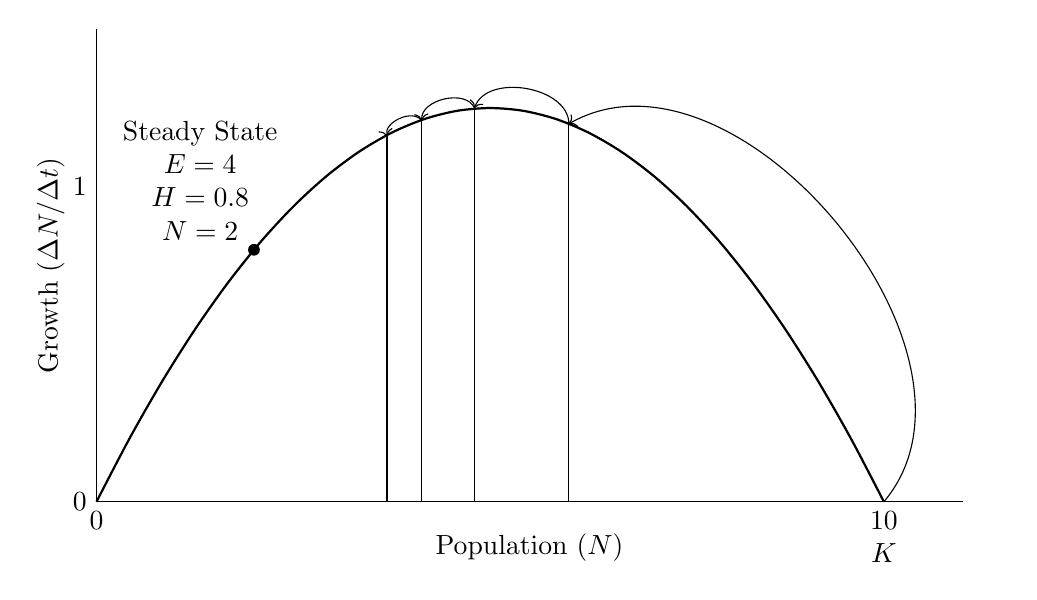
\begin{tikzpicture}
		\draw [-] (0,0) to node [below, yshift=-8pt] {Population ($N$)} (11,0);
		\draw [-] (0,0) to node [above, sloped, yshift=8pt] {Growth ($\Delta N / \Delta t$)} (0,6);
		\draw [thick, domain=0:10, smooth, variable=\N] plot ({\N},{4*(0.5*\N*(1-\N/10))});
		\node [below, align=center] at (10,0) {$10$ \\ $K$};
		\node [below] at (0,0) {0};
		\node [left] at (0,0) {0};
		\node [left] at (0,4) {1};
		\draw [-, thin] (6,0) to (6,4.8);
		\draw [-, thin] (4.8,0) to (4.8,5);
		\draw [-, thin] (4.13,0) to (4.13,4.84);
		\draw [-, thin] (3.69,0) to (3.69,4.64);
		\node[circle, fill=black, inner sep=1.5pt] at (2,3.2) {};
		\node[align=center, above left, xshift=12pt] at (2,3.2) {Steady State \\ $E=4$ \\ $H=0.8$ \\ $N=2$};
		\draw [->, thin] (10,0) to [bend right=80] (6,4.8);
		\draw [->, thin] (6,4.8) to [bend right=80] (4.8,5);
		\draw [->, thin] (4.8,5) to [bend right=80] (4.13,4.84);
		\draw [->, thin] (4.13,4.84) to [bend right=80] (3.69,4.64);
	\end{tikzpicture}
\end{frame}

\begin{frame}{Fishing Sustainably}
	\begin{itemize}
		\item Starting from fish population $N = 10$:
		\item Effort $E=4$ leads to:
		\begin{itemize}
			\item An immediate harvest of $H = 4$ 
			\item A steady state with $N = 2$ and $H = 0.8$
		\end{itemize} 
		\item Effort $E=2$ leads to:
		\begin{itemize}
			\item An immediate harvest of $H = 2$ 
			\item A steady state with $N = 6$ and $H = 1.2$
		\end{itemize} 
		\item Steady states are "sustainable", in that the activities can continue indefinitely.
		\item Is one steady state better?
		\item Can it be better to take big harvests in the early years, ending up with a lower sustainable harvest?
	\end{itemize}
\end{frame}

\mode<article>{
	Each effort level corresponds to a unique steady state, or sustainable, stock and harvest level.  These combinations are shown in the figure.  Notice that the curve has the same shape as the stock and growth curve.  However, the horizontal axis represents the effort devoted to fishing, and the vertical axis the harvest.  The higher the effort level, the lower the corresponding steady state stock.  The stock will be at its carrying capacity when there is no effort, when no fish are being harvested.  With high enough effort, all the fish will be caught and the stock will be driven to zero.
	
	Is an effort level that drives the stock to zero sustainable?  Seems strange to consider.  However, if the stock is zero and therefore the harvest is zero, this will continue to be the case into the future.  In a strange way, a fish stock that has been driven to extinction is now sustainable, as it is not changing any more.
	
	This highlights that when we talk about sustainability, we are not just talking about a technical state of a system.  Sustainability as a concept, in most of the ways that we use the idea, is not the same thing as a steady state.  There is something more to it.
}

\begin{frame}{Fishing Sustainably}
	\begin{tikzpicture}
		\draw [-] (0,0) to node [below, yshift=-8pt] {Effort ($E$)} (11,0);
		\draw [-] (0,0) to node [above, sloped, yshift=8pt] {Harvest $H = \Delta N / \Delta t$} (0,6);
		\draw [domain=0:10, smooth, variable=\E] plot ({\E},{4*10*0.1*(\E/2)*(1-0.1*(\E/2)/0.5))});
		\node [below, align=center] at (10,0) {5};
		\node [below] at (0,0) {0};
		\node [left] at (0,0) {0};
		\node [left] at (0,4) {1};
		\node [right, align=left] at (7,5.5) {$H = 10\times 0.1E \left(1-\dfrac{0.1}{0.5}E\right)$};
		\draw [-, thin, dashed] (0,5) to (5,5) to (5,0);
		\node [below] at (5,0) {2.5};
		\node [left] at (0,5) {1.25};
	\end{tikzpicture}
\end{frame}

\begin{frame}{Fishing Sustainably}
	\begin{itemize}
		\item Each effort level corresponds with a steady state "sustainable" stock size and harvest level.
		\item There is one effort level that corresponds to the maximum sustainable harvest.
		\begin{itemize}
			\item In the fisheries literature, this is the \textit{\textbf{maximum sustainable yield (MSY)}}.
		\end{itemize}
		\item When is it best to manage a resource to achieve the maximum sustainable yield?
		\item What is the \textit{\textbf{function}} of this harvester and fish pond system?
		\item What would it mean for this harvester and fish pond system to be \textit{\textbf{resilient}}?
	\end{itemize}
\end{frame}


	
	\chapter{Social Ecological Systems \#2}
	%! TEX root = ../notes/main_notes.tex

\lecture{A Foundational Social Ecological System}{lec-SES2}

\mode<article>{
	Sustainability challenges exist because of the interaction between humans and the environment they inhabit.
	
	Lets consider a system that incorporates humans and the environment.
	
	A simple example is a 'stylized' hunter gatherer model.  In this case, our hunters will harvest fish, building on the model considered earlier.
}

\begin{frame}{The Hunter Gatherer Village}
	\begin{itemize}
		\item The Question: ?
		\begin{itemize}
			\item 1
		\end{itemize}
	\end{itemize}
\end{frame}

\mode<article>{
	An apparently simple mode can become complex pretty quickly.
}

\begin{frame}{The Hunter Gatherer Village}
	\centering
	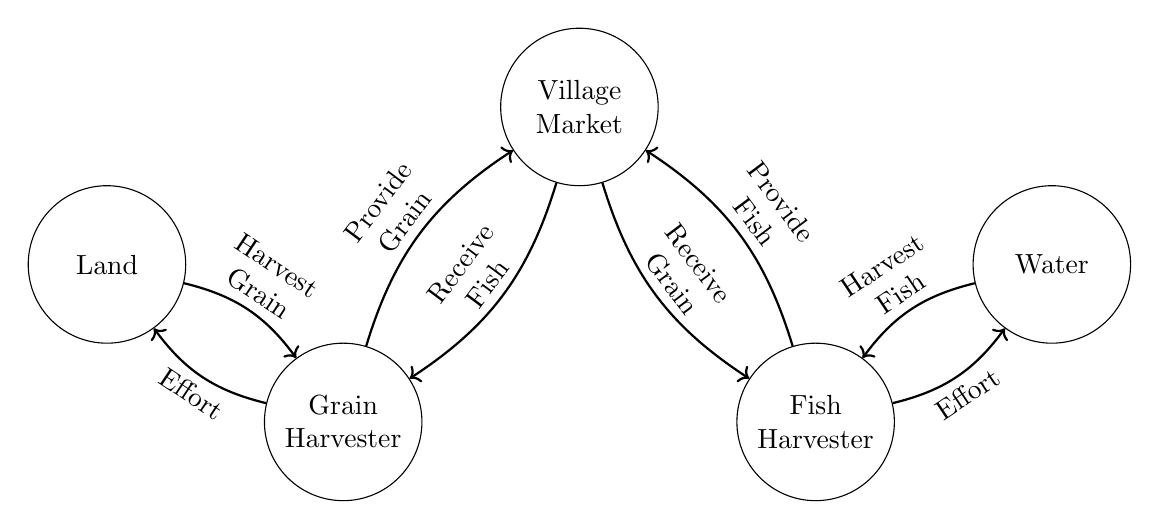
\begin{tikzpicture}
		% Define and place the nodes
		\node [circle, draw, minimum size=2cm, align=center] at (6,6) (village) {Village \\ Market};
		\node [circle, draw, minimum size=2cm, align=center] at (3,2) (gather) {Grain \\ Harvester};
		\node [circle, draw, minimum size=2cm, align=center] at (9,2) (fish) {Fish \\ Harvester};
		\node [circle, draw, minimum size=2cm, align=center] at (0,4) (land) {Land};
		\node [circle, draw, minimum size=2cm, align=center] at (12,4) (water) {Water};
		
		% Draw edges
		\draw [->, thick, align=center] (land) to [bend left=20] node [above, sloped] {Harvest \\ Grain} (gather);
		\draw [->, thick, align=center] (gather) to [bend left=20] node [below, sloped] {Effort} (land);
		\draw [->, thick, align=center] (water) to [bend right=20] node [above, sloped] {Harvest \\ Fish} (fish);
		\draw [->, thick, align=center] (fish) to [bend right=20] node [below, sloped] {Effort} (water);
		\draw [->, thick, align=center] (gather) to [bend left=20] node [above, sloped] {Provide \\ Grain} (village);
		\draw [->, thick, align=center] (village) to [bend left=20] node [above, sloped] {Receive \\ Fish} (gather);
		\draw [->, thick, align=center] (fish) to [bend right=20] node [above, sloped] {Provide \\ Fish} (village);
		\draw [->, thick, align=center] (village) to [bend right=20] node [above, sloped] {Receive \\ Grain} (fish);
	\end{tikzpicture}
\end{frame}

\begin{frame}{The Hunter Gatherer Village}
	\begin{itemize}
		\item The grain subsystem
		\begin{itemize}
			\item Grain grows on the land
			\item Grain harvesters exert effort that translates into harvested grain.
		\end{itemize}
		\item The fish subsystem
		\begin{itemize}
			\item Fish grow in the water
			\item Fish harvesters exert effort that translates into harvested fish.
		\end{itemize}
		\item The Village system
		\begin{itemize}
			\item Fish harvesters bring fish to the village, receive grain.
			\item Grain harvesters bring grain to the village, receive fish.
			\item How is the exchange of fish for grain managed?
		\end{itemize}
	\end{itemize}
\end{frame}


	
	\backmatter
	% Optional: Bibliography or Index
	% \printbibliography
	
\end{document}